\documentclass[12pt]{article} % размер шрифта

\usepackage{tikz} % картинки в tikz
\usepackage{microtype} % свешивание пунктуации

\usepackage{array} % для столбцов фиксированной ширины

\usepackage{indentfirst} % отступ в первом параграфе

\usepackage{multicol} % текст в несколько колонок
\usepackage{verbatim}

\graphicspath{{images/}} % путь к картинкам

\usepackage{sectsty} % для центрирования названий частей
\allsectionsfont{\centering} % приказываем центрировать все sections

\usepackage{amsmath, amssymb} % куча стандартных математических плюшек

\usepackage[top=2cm, left=1.5cm, right=1.5cm, bottom=2cm]{geometry} % размер текста на странице

\usepackage{lastpage} % чтобы узнать номер последней страницы

\usepackage{enumitem} % дополнительные плюшки для списков
%  например \begin{enumerate}[resume] позволяет продолжить нумерацию в новом списке
\usepackage{caption} % подписи к картинкам без плавающего окружения figure


\usepackage{fancyhdr} % весёлые колонтитулы
\pagestyle{fancy}
\lhead{ФМТ}
\chead{}
\rhead{КЛШ-2019}
\lfoot{}
\cfoot{}
\rfoot{\thepage/\pageref{LastPage}}
\renewcommand{\headrulewidth}{0.4pt}
\renewcommand{\footrulewidth}{0.4pt}



\usepackage{todonotes} % для вставки в документ заметок о том, что осталось сделать
% \todo{Здесь надо коэффициенты исправить}
% \missingfigure{Здесь будет картина Последний день Помпеи}
% команда \listoftodos — печатает все поставленные \todo'шки

\usepackage{booktabs} % красивые таблицы
% заповеди из документации:
% 1. Не используйте вертикальные линии
% 2. Не используйте двойные линии
% 3. Единицы измерения помещайте в шапку таблицы
% 4. Не сокращайте .1 вместо 0.1
% 5. Повторяющееся значение повторяйте, а не говорите "то же"

\usepackage{fontspec} % поддержка разных шрифтов
\usepackage{polyglossia} % поддержка разных языков

\setmainlanguage{russian}
\setotherlanguages{english}

\setmainfont{Linux Libertine O} % выбираем шрифт
% можно также попробовать Helvetica, Arial, Cambria и т.Д.

% чтобы использовать шрифт Linux Libertine на личном компе,
% его надо предварительно скачать по ссылке
% http://www.linuxlibertine.org/

\newfontfamily{\cyrillicfonttt}{Linux Libertine O}
% пояснение зачем нужно шаманство с \newfontfamily
% http://tex.stackexchange.com/questions/91507/

\AddEnumerateCounter{\asbuk}{\russian@alph}{щ} % для списков с русскими буквами
\setlist[enumerate, 2]{label=\asbuk*),ref=\asbuk*} % списки уровня 2 будут буквами а) б) ...

%% эконометрические и вероятностные сокращения
\DeclareMathOperator{\Cov}{Cov}
\DeclareMathOperator{\Corr}{Corr}
\DeclareMathOperator{\Var}{Var}
\DeclareMathOperator{\E}{\mathbb{E}}
\def \hb{\hat{\beta}}
\def \hs{\hat{\sigma}}
\def \htheta{\hat{\theta}}
\def \s{\sigma}
\def \hy{\hat{y}}
\def \hY{\hat{Y}}
\def \v1{\vec{1}}
\def \e{\varepsilon}
\def \he{\hat{\e}}
\def \z{z}
\def \hVar{\widehat{\Var}}
\def \hCorr{\widehat{\Corr}}
\def \hCov{\widehat{\Cov}}
\def \cN{\mathcal{N}}
\let\P\relax
\DeclareMathOperator{\P}{\mathbb{P}}
\let\Re\relax
\DeclareMathOperator{\Re}{Re}



\begin{document}

\section*{Вступление}

Дорогой Друг! Это задачи физмат-турнира клш-2019. Решай их и готовься к новому сезону! 
Если у тебя есть вопросы по задачам, можешь написать Никите Астраханцеву (телеграм \verb|@nikita_astronaut|) или Боре Демешеву (телеграм \verb|@boris_demeshev|).

Начиная с третьего тура верхние три стола получали чуть более сложную версию одной задачи. 
Эта задача отмечена звёздочкой. 

\section*{Жеребьёвка}

\begin{enumerate}
    \item {[Математика 1б]} Иванушка-Дурачок начертил выпуклый многоугольник, 
    провёл в нём все диагонали и нашёл сумму числа сторон и диагоналей. Она оказалась равной 6. 
    Какой многоугольник начертил Иванушка?
    \item {[Математика 1б]} Найди угол между двумя медианами в равностороннем треугольнике.
    \item {[Физика 1б]} Автомобиль проходит первую половину пути со скоростью 100 км/ч, а вторую — со скоростью 60 км/ч. 
    Какова его средняя скорость?
    \item {[Физика 1б]} Две одинаковые пружины с коэффициентом жёсткости $k$ каждая соединены последовательно. 
    Найди коэффициент жёсткости пружины, получившейся в результате соединения.
    \item {[Математика 2б]} На некотором острове 2/3 всех мужчин женаты и 3/5 всех женщин замужем. 
    Какая доля населения острова состоит в браке? На этом острове браком называется союз одного мужчины и одной женщины.
    \item {[Физика 2б]} Маятник в ускоряющемся поезде отклоняется от вертикали на угол $30^{\circ}$. Найди
    ускорение поезда.
    \item {[Математика 3б]} Василиса Премудрая нашла расстояние между серединами диагоналей заколдованной трапеции 
    с основаниями $a$, $b$, где $a < b$. Что она получила? 
    
    Примечание: Василиса тренировалась решать задачи в КЛШ и никогда не делает ошибок.
    \item {[Физика 3б]} Илья Муромец бросает резиновую булаву́ с дерева высоты $h$ вниз под углом
    $\alpha$ к горизонту со скоростью $v$. 
    
    На какую максимальную высоту над землёй подскочит булава́ после абсолютно упругого удара о землю?
    \item {[Математика 4б]} Неопознанная шахматная фигура (НШФ) может ходить по шахматной доске только на одну клетку вверх или направо 
    (не по диагонали!). Сколькими различными способами НШФ может дойти из левого нижнего угла 
    до правого верхнего угла шахматной доски?
    \item {[Физика 4б]} Первая электроплитка рассчитана на напряжение 220 В и имеет мощность 1 кВт,
    а вторая, рассчитанная на то же напряжение, имеет мощность 1.5 кВт. 
    Сколько процентов составляет мощность первой плиты от мощности второй, 
    если их соединить последовательно в сеть напряжением 220 В? 
    
    Зависимостью сопротивления от температуры пренебречь.
\end{enumerate}

\section*{Демо-тур}

\begin{enumerate}
\item Иван Царевич сел на ковёр-самолёт. Пролетев половину всего пути, он заснул и спал до тех пор, 
пока не осталось пролететь половину того пути, который он проспал. 
Проснувшись, он долетел до пункта назначения бодрствующим. Какую часть всего пути Иван пролетел бодрствующим? 

\item Воздушный шар опускался с постоянной скоростью. Когда из него выбросили груз массой $m$, 
он начал подниматься с той же скоростью. Найди силу сопротивления воздуха при этой скорости.



%\item[3] Имеется треугольник с целочисленными сторонами; известно, что его стороны составляют арифметическую прогрессию со знаменателем 13. Чему равен наименьший периметр такого треугольника?
%\bigskip
%\\
%Ответ: $14+27+40=81$


\item 
\begin{minipage}{\linewidth}
        \centering
        \begin{minipage}{0.60\linewidth}
                Известно, что точка $C$ лежит на прямой $c$. Найди наименьшее возможное значение суммы расстояний $AC+CB$. 
                Сторона каждой клетки равна 1.
        \end{minipage}
        \hspace{0.05\linewidth}
        \begin{minipage}{0.3\linewidth}
        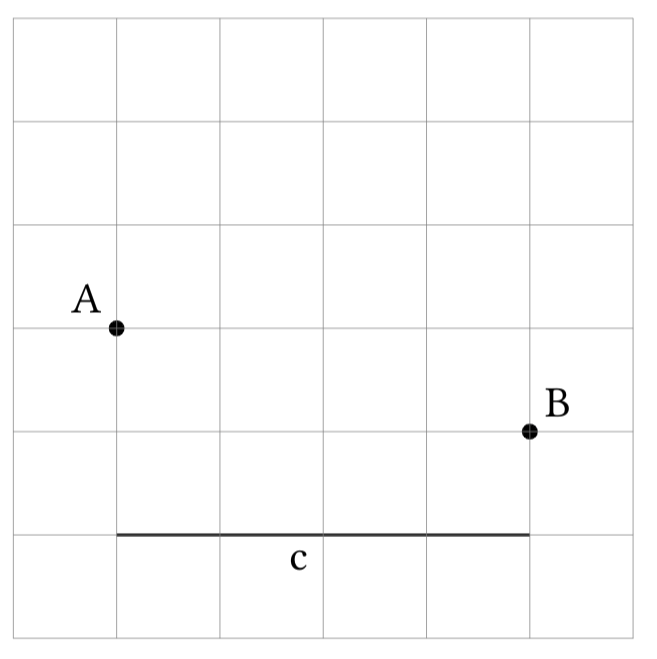
\includegraphics[scale=0.2]{lattice.png}
            
        \end{minipage}
    \end{minipage}



\item Максимальное и минимальное ускорения автомобиля равны $a_0$ и $-a_0$, соответственно. 
За какое наименьшее время автомобиль может, начав из состояния покоя, прибыть в точку назначения с нулевой скоростью, 
если расстояние до точки назначения равно $d$?

\end{enumerate}
    



\section*{Тур 1}


\begin{enumerate}
\item Какое число нужно вычесть из числителя дроби $537/463$ и прибавить к знаменателю, 
чтобы после сокращения получить $1/9$?

\item
Илон Маск стоит на горизонтальной плоскости и бросает камень под углом $\alpha$  горизонту со скоростью $v$. 
Через какое время камень впервые будет находиться на высоте $3 v^2 \sin^2 \alpha / (8 g)$? 
Ускорение свободного падения равно $g$. 

\item
В квадрат со стороной $a$ вписана окружность $\Omega$. 
Окружность $\omega$ касается ровно двух сторон квадрата и окружности $\Omega$. Найди радиус окружности $\omega$.

\item
\begin{minipage}{\linewidth}
        \centering
        \begin{minipage}{0.60\linewidth}
        Груз массы $M$ подвешен на пяти блоках, как показано на рисунке. 
        Трения в блоках нет, масса нити и блоков пренебрежимо мала по сравнению с массой груза. 
        Угол между нитями, расходящимися под углом от подвижного блока на грузе, составляет $120^{\circ}$. 
        Найди натяжение $T$ нити.
        \end{minipage}
        \hspace{0.05\linewidth}
        \begin{minipage}{0.3\linewidth}
            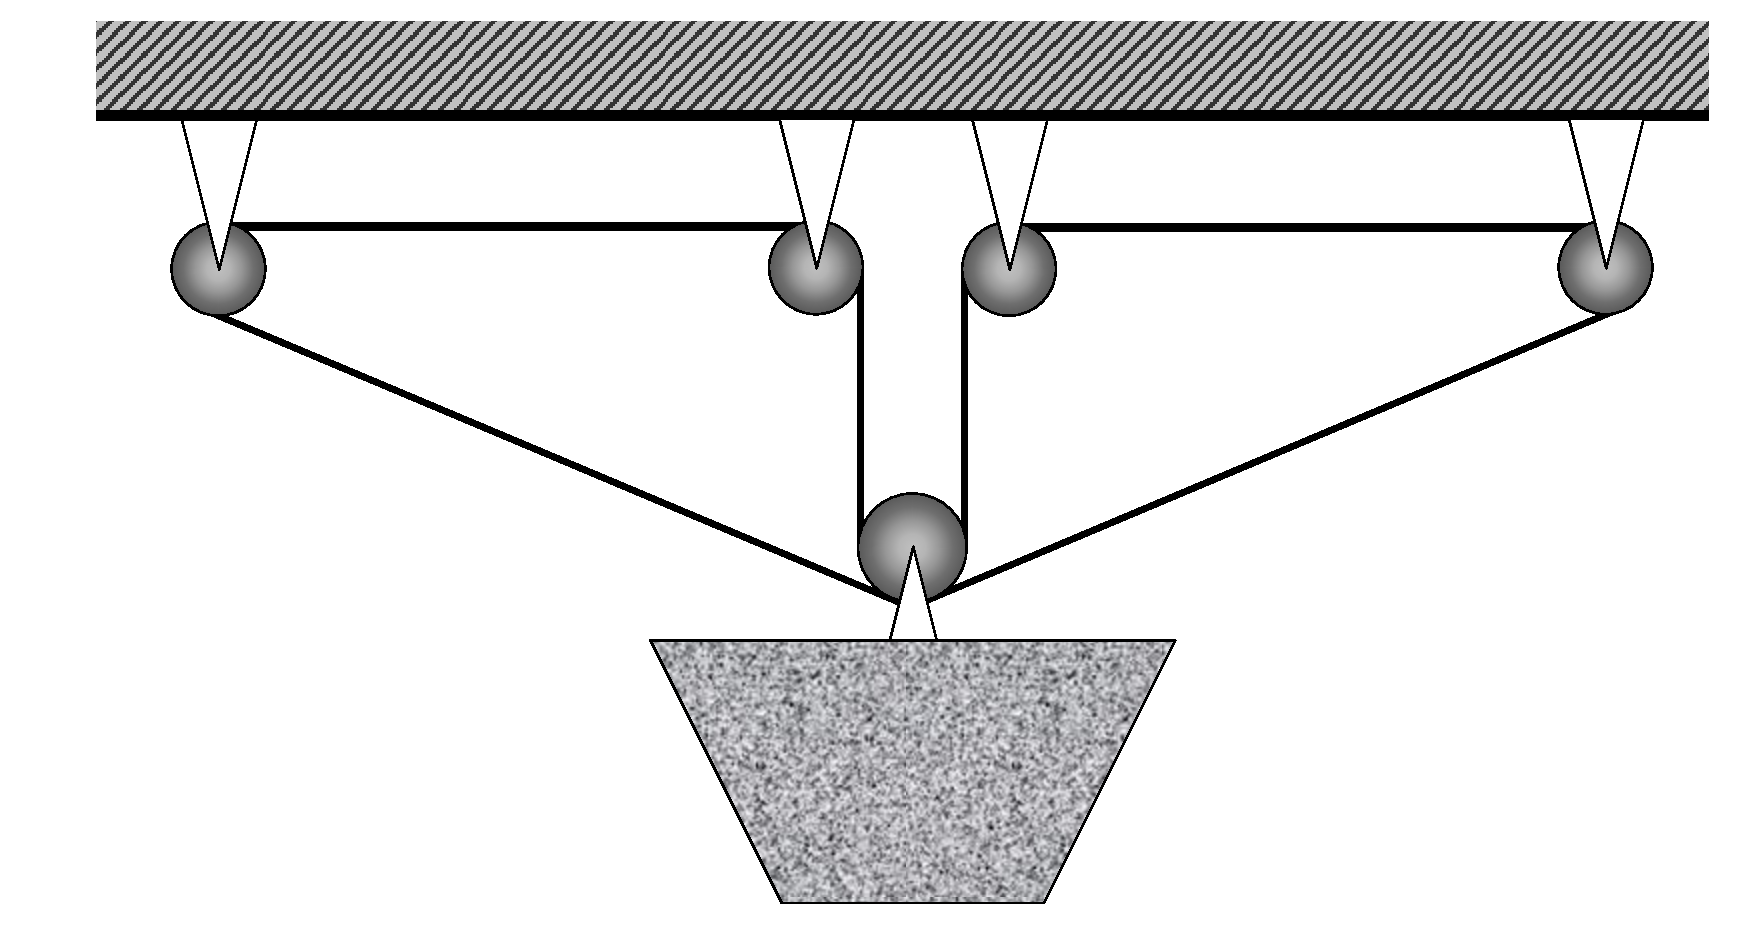
\includegraphics[scale=0.2]{fig2_tmp.pdf}
        \end{minipage}
    \end{minipage}


\end{enumerate}
    
\section*{Тур 2}

\begin{enumerate}
\item Сколько существует различных треугольников с целочисленными сторонами и периметром 13?

\item Илон Маск находится на горизонтальной плоскости и бросает камень под углом $\alpha$ к горизонту со скоросью $v$. 
В тот момент, когда камень находится в наивысшей точке, он неупруго ударяется о покоящийся вертикальный шаттл Space-X, 
теряет половину своей кинетической энергии и отскакивает обратно в сторону Илона. 
На каком расстоянии от Илона Маска упадёт камень? Ускорение свободного падения равно $g$.


\item
\begin{minipage}{\linewidth}
        \centering
        \begin{minipage}{0.78\linewidth}
        Вокруг треугольника $\bigtriangleup ABC$ со сторонами $AB = AC = 4$, $BC = 2$ описана окружность $\Omega$. 
        Окружность $\omega$ касается окружности $\Omega$ и середины стороны $BC$. Найди радиус окружности $\omega$.
        \end{minipage}
        \hspace{0.05\linewidth}
        \begin{minipage}{0.15\linewidth}
            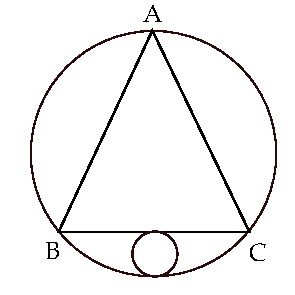
\includegraphics[scale=0.5]{drawing.pdf}
        \end{minipage}
    \end{minipage} 


\item
По горизонтальной плоскости скользит шайба, коэффициент трения между шайбой и плоскостью равен $\mu$. 
Пройдя путь $L$, шайба останавливается. Чему равна начальная скорость шайбы? Ускорение свободного падения равно $g$.

\end{enumerate}
    


\section*{Тур 3}


\begin{enumerate}
\item Требуется разложить 8 кусков сахара в 4 одинаковых стакана так, чтобы в каждом стакане лежал хотя бы один кусок. 
Сколько различных раскладок существует? Раскладки не являются различными, 
если они могут быть получены друг из друга перестановкой стаканов.

\item[1*.] Сколько существует различных треугольников с целочисленными сторонами и периметром 100?


\item 
\begin{minipage}{\linewidth}
        \centering
        \begin{minipage}{0.65\linewidth}
                В автомобиле Tesla Model S используется современная электросхема, приведённая на рисунке. 
                Сопротивление всех сегментов показано на рисунке. Илон Маск решил узнать эквивалентное сопротивление между точками $A$ и $B$. 
                Чему оно равно?
        \end{minipage}
        \hspace{0.05\linewidth}
        \begin{minipage}{0.25\linewidth}
            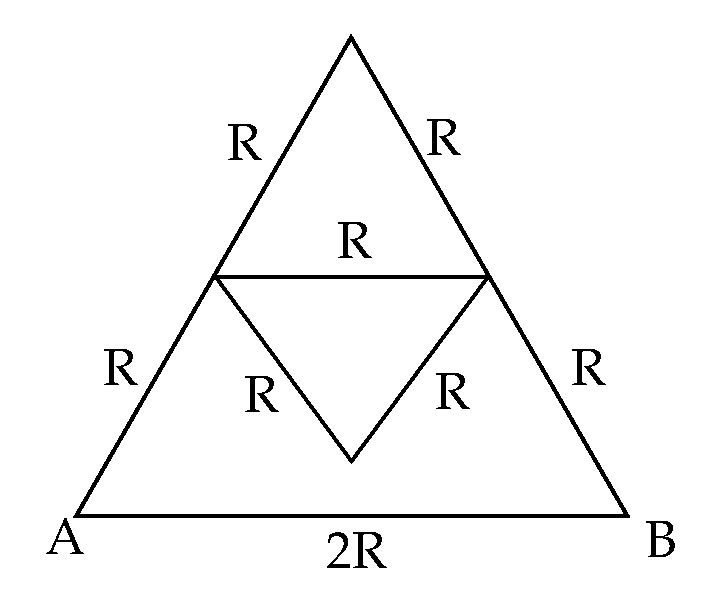
\includegraphics[scale=0.4]{drawing-1.pdf}
        \end{minipage}
    \end{minipage} 

\item  Дана окружность радиуса $R$. Точки $A$, $B$, $C$ на ней делят её на дуги, длины которых относятся как $3:4:5$. 
В этих точках к окружности проведены касательные, точки пересечения которых образуют треугольник. 
Найди площадь этого треугольника.

\item По горизонтальной плоскости скользит шайба массы $M$, коэффициент трения между шайбой и плоскостью равен $\mu$, 
ускорение свободного падения $g$. Пройдя путь $L$, шайба ударяется о вертикально стоящую стенку, 
теряя половину кинетической энергии, и останавливается в исходной точке. Чему равна начальная скорость $v_0$ шайбы?

\end{enumerate}
    


\section*{Тур 4}

\begin{enumerate}
\item Функция $f(x)$ задаётся уравнением $3f(x) + f(-x) = x^2 + 2x$. Чему равно $f(2)$?

\item
\begin{minipage}{\linewidth}
        \centering
        \begin{minipage}{0.58\linewidth}
        Все рёбра октаэдра имеют сопротивление $R$. Найди сопротивление между точками $A$ и $B$.
        \end{minipage}
        \hspace{0.05\linewidth}
        \begin{minipage}{0.15\linewidth}
            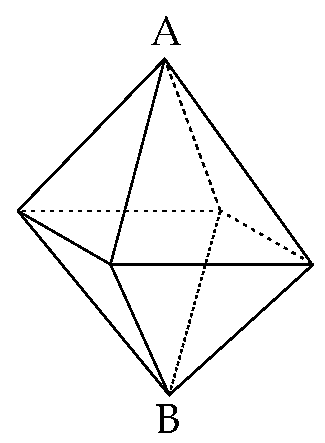
\includegraphics[scale=0.4]{resistors_octo.pdf}
        \end{minipage}
    \end{minipage} 

\item Радиусы двух окружностей равны $27$ и $13$. Расстояние между центрами окружностей равно $50$. 
Найди длину отрезка общей касательной. Упрости ответ полностью.

\item
Два одинаковых больших резервуара заполнены объёмом $V$ жидкости, температура жидкости в первом резервуаре $T$, 
во втором $2 T$. Ковшом объёма $V / 5$ зачерпывают жидкость из первого резервуара и переливают во второй. 
Затем этим же ковшом зачерпывают воду из второго резервуара и переливают в первый. 
Найди отношение температуры в первом резервуаре к температуре во втором резервуаре после такого переливания. 
Теплоёмкостью ковша, резервуаров и теплообменом с окружающей средой пренебреги. 
При переливании ковш полностью заполняется водой.

\item[4*.]
Два одинаковых больших резервуара заполнены объёмом $V$ жидкости, температура жидкости в первом резервуаре $T$, 
во втором $2 T$. Ковшом объёма $V / 5$ зачерпывают жидкость из первого резервуара и переливают во второй. 
Затем этим же ковшом зачерпывают воду из второго резервуара и переливают в первый. Эту процедуру, 
состоящую из двух переливаний, повторяют ещё $N - 1$ раз. Найди разность температур во втором и первом резервуарах после такого переливания. 
Теплоёмкостью ковша, резервуаров и теплообменом с окружающей средой пренебреги. При переливании ковш полностью заполняется водой.



\end{enumerate}
    


\section*{Тур 5}

\begin{enumerate}
\item В столбик выписали все десятизначные числа, кратные 9 и записывающиеся только нулями и единицами. 
Чему равна их сумма? 

\item За 2 секунды прямолинейного равноускоренного движения тело прошло 20 метров, увеличив свою скорость в 3 раза. 
Определи начальную скорость тела.

\item В треугольнике $\bigtriangleup ABC$ точки $N,\,M,\,K$ лежат на сторонах $AC,\,AB,\,BC$, соответственно. 
Отрезок $NK$ параллелен $AB$, отрезок $MN$ параллелен $BC$. Известно, что $S_{\bigtriangleup AMN} = S_1$, 
$S_{\bigtriangleup NKC} = S_2,$ найди площадь $S_{MNKB}$.

\item На абсолютно гладкой горизонтальной поверхности лежат два груза массы $M_1 = 1$\,кг и $M_2 = 2$\,кг. 
Они связаны тонкой нерастяжимой невесомой нитью. Груз массой $M_2$ тянут в направлении {\bf от} груза $M_1$ с силой $F = 12$\,Н. 
Найди натяжение нити.

\item[4*.] На горизонтальной поверхности лежат подряд лежат $N$ грузов массами $1$\,кг, $2$\,кг, $\ldots$, $N$\,кг. 
Коэффициент трения между грузами и поверхностью $\mu$. Грузы связаны тонкими невесомыми нитями. 
Груз массой $1$\,кг тянут в направлении {\bf от} остальных грузов с силой $F$. 
Найди натяжение нити между грузами масс $N - 1$\,кг и $N$\,кг.


\end{enumerate}
    


\section*{Тур 6}

\begin{enumerate}
\item Запиши значение выражения $\sqrt{8 + 2\sqrt{8 + 2\sqrt{8 + 2\sqrt{\ldots}}}}$ в виде целого числа.

\item Тело упало в ущелье с Рейхенбахского водопада. Весь полет занял время $t$. 
За какое время тело пролетело последнюю треть высоты? Считай, что тело падало из состояния покоя. 
Сопротивлением воздуха пренебреги.

\item Сторона $AO$ треугольника $\bigtriangleup ADO$ равна 36. Прямая, параллельная этой стороне, 
делит треугольник на две равновеликие части. Найди длину отрезка этой прямой, заключённого между сторонами треугольника.

\item Два шарика массами $m$ и $2m$ подвешены на длинных нитях так, что они соприкасаются и
их центры масс находятся на одной высоте. Шарик массы $m$ отводят в сторону на натянутой нити, 
поднимая его на высоту $H$, и отпускают. 
Какое количество тепла выделится при абсолютно неупругом центральном соударении шариков? 
Ускорение свободного падения равно~$g$.

\item[4*.] Два шарика массами $m$ и $2m$ подвешены на длинных нитях так, 
что они соприкасаются и их центры масс находятся на одной высоте. 
Шарик массы $m$ отводят в сторону на натянутой нити, поднимая его на высоту $H$, и отпускают. 
Шарики сталкиваются абсолютно упруго. 
Найди, на сколько максимальная высота подъёма шарика массы $2 m$ окажется больше максимальной высоты подъёма шарика массы $m$.


\end{enumerate}
    


\section*{Свалка}


\begin{enumerate}
\item В своём письме домой школьник написал: «Наш {\it обычный обед} состоит на 50\,\% из гарнира, 
на 20\,\% из рыбных котлет и на 30\,\% из {\it обычного обеда}». Найди, какую долю гарнир составляет в обычном обеде.

\item
В схеме на рисунке все сопротивления равны $R$. Найди сопротивление между точками $A$ и $B$.
\begin{figure}[h!]
\center
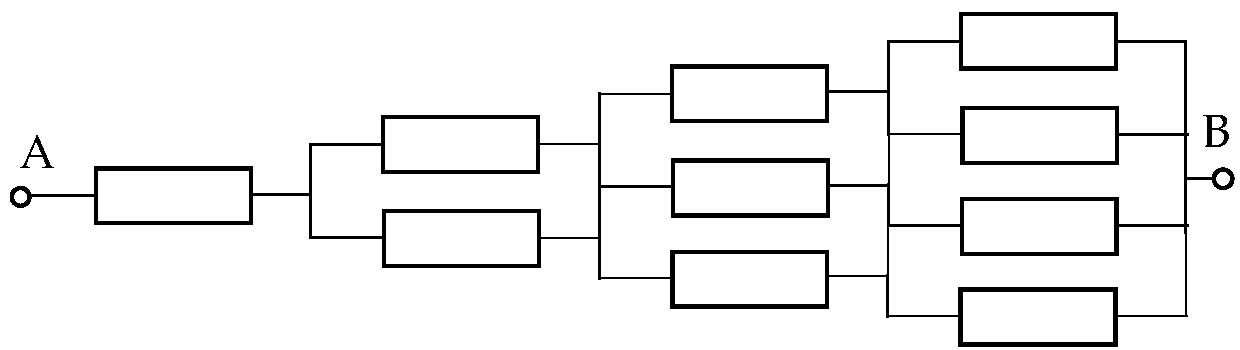
\includegraphics[scale=0.3]{resistors_1234.pdf}
\end{figure}

\item Дана трапеция $LAMZ$ с основаниями $AM = 4$ и $LZ = 16$, 
в которую можно вписать окружность и вокруг которой можно описать окружность. Найди произведение их радиусов.

\item Материальная точка начинает двигаться из состояния покоя по прямой с постоянным ускорением. 
Спустя время $\tau$ после начала её движения ускорение меняет знак на противоположный, оставаясь неизменным по модулю. 
Определи, через какое время {\bf после начала движения} точка окажется в исходном положении?

\end{enumerate}



\section*{Финал}

\begin{enumerate}
\item Сторона куба равна 5. В центре каждой грани куба вырезают квадратную дырку размером $2 \times 2$. 
Дырки сквозные, их стороны параллельны соответствующим рёбрам куба. Найди объем оставшейся части куба.

\item Рыбак находится на льдине, верхняя поверхность льдины находится над водой. 
Льдина имеет вид вертикального цилиндра. Определи наименьшую возможную площадь льдины, если масса рыбака — $m$, 
а толщина льдины — $h$. Плотность воды равна $\rho_1$, плотность льда — $\rho_2$, где $\rho_1 > \rho_2$. 
Ускорение свободного падения равно $g$.

\item В треугольнике $\bigtriangleup ABC$ сторона $BC$ равна $2 \sqrt{3} / 3$. 
Медианы треугольника $A A_1$,\,$B B_1$,\,$C C_1$ пересекаются в точке $O$, и известно, 
что точки $O$,\,$B_1$,\,$C_1$,\,$A$ лежат на одной окружности. Найди длину медианы $A A_1$.

\item Подвешенному на нити шарику сообщили начальную скорость в горизонтальном направлении. 
Когда нить отклонилась на угол $\alpha = \pi/6$ от вертикали, ускорение шарика оказалось направленным горизонтально. 
Найди $\cos\beta$, где $\beta$ — это угол максимального отклонения~нити.

\end{enumerate}
    

\section*{Ответы}

\subsection*{Жеребьёвка}

\begin{enumerate}
\item четырёхугольник или более точно «выпуклый четырёхугольник». Ответ «квадрат» или «прямоугольник» не принимается.
\item $120^{\circ}$ или $60^{\circ}$ или $2\pi/3$ или $\pi/3$
\item 75 км/ч
\item $k/2$
\item $12/19$
\item $g/ 3 = g \sqrt{3}/3$
\item $(b − a)/2$
\item $h + v^2 \sin^2 \alpha/2g$
\item $C_{14}^7 = 14!/(7!)^2=3432$. Просто ответ $C_{14}^7$ не принимался, только ответ с факториалами или числом. 
\item $150\%$
\end{enumerate}


\subsection*{Демо-тур}

\begin{enumerate}
\item $2/3$
\item $mg/2$
\item $5$
\item $2\sqrt{d/a_0}$
\end{enumerate}

\subsection*{Тур 1}

\begin{enumerate}
\item $437$: замечаем, что $1/9=100/900$, в числителе перебор на 437, в знаменателе аналогичный недобор.
\item 
\item $\sqrt{34}$
\item $T=Mg/3$
\end{enumerate}

\subsection*{Тур 2}

\begin{enumerate}
\item $5$: перебираем по длинной стороне. Находим: $6-6-1$, $6-5-2$, $6-4-3$, $5-5-3$, $5-4-4$.
\item 
\item 
\item 
\end{enumerate}

\subsection*{Тур 3}

\begin{enumerate}
\item $5$: перечисляем по самому заполненному стакану. Для удобства приклеим четыре куска сразу ко дну каждого стакана. 
Итого: $4-0-0-0$, $3-1-0-0$, $2-2-0-0$, $2-1-1-0$, $1-1-1-1$.
\item 
\item 
\item 
\item 
\end{enumerate}

\subsection*{Тур 4}

\begin{enumerate}
\item Подставляем $2$ и $-2$ вместо $x$. Получаем $f(2)=3$.
\item 
\item 
\item 
\item 
\end{enumerate}

\subsection*{Тур 5}

\begin{enumerate}
\item 
\item 
\item 
\item 
\item 
\end{enumerate}

\subsection*{Тур 6}

\begin{enumerate}
\item 
\item 
\item 
\item 
\item 
\end{enumerate}


\subsection*{Свалка}

\begin{enumerate}
\item $5/7$
\item $25R/12$ 
\item $5\sqrt{41}$ 
\item $t(2 + \sqrt 2)$
\end{enumerate}
    
\subsection*{Финал}

\begin{enumerate}
\item вырезаемая часть куба равна $60 - 16 = 44$, оставшая часть куба равна  $125 - 44 = 81$
\item 
\[ 
    mg + \rho_2 h Sg = \rho_1 h S g
\]
\[
    S = \frac{m}{h(\rho_1 - \rho_2)}
\]
\item Углы $\angle OAB_1$ и $\angle OC_1B$ равны. Опираются на одну дугу. 

Треугольники $\triangle OA_1C$ и $\triangle CA_1A$ подобны.

Пусть $OA_1 = x$, $BC = a$, тогда 

\[
\frac{x}{a/2} = \frac{a/2}{3x}  
\]

$a = 2\sqrt{3}x$

$x=1/3$

Ответ: 1.

\item Второй закон Ньютона:
\[
\frac{mv^2}{R} = T - mg \frac{\sqrt{3}}{2} 
\]
Горизонтальное ускорение:
\[
mg = T \frac{\sqrt{3}}{2}  
\]
Получаем 
\[
\frac{v^2}{R} = \frac{2g}{\sqrt{3}} - g \frac{\sqrt{3}}{2}  
\]

Закон сохранения энергии
\[
\frac{v^2}{2} +gR\left(1- \cos \frac{\pi}{6} \right)  = gR(1-\cos\beta)  
\]
Делим на $R/2$ и подставляем:
\[
\frac{v^2}{R} +2g(1- \sqrt{3}/2)  = 2g(1-\cos\beta)  
\]

Итого

\[
\frac{2}{\sqrt{3}} - \frac{\sqrt{3}}{2} - \sqrt{3} = -2\cos\beta  
\]

\[
\cos\beta = \frac{5\sqrt{3}}{12}
\]

\end{enumerate} 
  



\end{document}
